\documentclass{article}
\usepackage[preprint]{neurips_2024}
\usepackage{amsmath,amssymb}
\usepackage{booktabs}
\usepackage{graphicx}
\usepackage{hyperref}
\usepackage{xcolor}
\usepackage{multirow}
\usepackage{enumitem}
\usepackage{url}

\hypersetup{
  colorlinks=true,
  linkcolor=blue!60!black,
  citecolor=green!50!black,
  urlcolor=blue!60!black
}

\title{HalluMaze: A Maze Navigation Benchmark\\for LLM Metacognitive Error Recovery}

\author{
  Jayone\\
  \texttt{https://github.com/jaytoone/HalluMaze}\\
  \texttt{https://huggingface.co/spaces/Be2Jay/hallumaze}
}

\date{}

\begin{document}
\maketitle

\begin{abstract}
We introduce \textsc{HalluMaze}, a benchmark that measures large language model (LLM) metacognitive error recovery through maze navigation.
Unlike existing hallucination benchmarks that evaluate final-answer accuracy, \textsc{HalluMaze} captures real-time error detection and corrective action by exposing models to navigable environments containing ``mirage'' walls---passages that appear blocked but are traversable.
We evaluate 13 LLMs across $n{=}60$ seeds $\times$ 5${\times}$5 and 7${\times}$7 maze sizes (780 total trials), including an extended evaluation of the Claude~4.x family (Haiku-4.5, Sonnet-4.5, Sonnet-4.6).
We introduce the \emph{Metacognitive Escape Index} (MEI), grounded in Nelson \& Narens' (1990) metamemory framework, which decomposes metacognitive performance into recovery rate (HRR), efficiency (ETR), awareness (AW), and error rate (HR).
All 13 tested LLMs score significantly below a random walk baseline ($p{<}0.001$ Bonferroni-corrected, $\delta{=}0.6$--$2.1$), revealing a systematic deficit in real-time metacognitive recovery.
Critically, we find that \emph{solve rate (SR) and metacognitive recovery (MEI/HRR) are orthogonal dimensions}: Claude-Sonnet-4.6 achieves the highest SR ($60\%$, rank~1) yet ranks~8th on MEI ($0.545$), while Claude-Sonnet-4.5 leads the leaderboard on MEI ($0.783$) with a more modest SR ($36.7\%$).
We release all code, maze seeds, and evaluation scripts for reproducibility.
\end{abstract}

% =================================================================
\section{Introduction}
% =================================================================

Large language models hallucinate---generating confident but factually incorrect outputs.
Prior work has measured hallucination at the response level: does the final answer contain errors? \citep{lin2022truthfulqa, ji2023halueval}.
However, metacognitive competence requires not just avoiding errors, but \textbf{detecting and recovering from them in real time}.

Consider a model navigating a maze.
It may hallucinate the existence of a wall, move into it, discover the contradiction when the environment responds, and then backtrack.
This sequence---error $\to$ detection $\to$ correction---is precisely the metacognitive loop that \citet{nelson1990metamemory} identify as the ``control'' function of metamemory.
No existing benchmark captures this.

\textbf{\textsc{HalluMaze}} fills this gap by embedding LLMs in a text-based maze navigation task where:
\begin{enumerate}[nosep]
  \item ``Mirage'' positions (hallucination traps) appear blocked but are traversable---the model must infer the error from contradictory environment feedback;
  \item Every step is logged, enabling real-time metacognitive signal extraction;
  \item Multiple metrics capture distinct metacognitive functions (monitoring vs.\ control).
\end{enumerate}

\noindent Our main findings:
\begin{itemize}[nosep]
  \item \textbf{All 13 tested LLMs score below random walk} on MEI ($p{<}0.001$, $\delta{=}0.6$--$2.1$).
  \item \textbf{Claude-Sonnet-4.5 leads the 13-model leaderboard} (MEI$=$0.783, SR$=$36.7\%, HRR$=$89.2\%). Among the original 10-model cohort, Claude-3.7-Sonnet leads (MEI$=$0.774, SR$=$56.7\%, HRR$=$87.5\%).
  \item \textbf{Frontier cost $\neq$ metacognition}: GPT-4o ranks last (MEI$=$0.315, HRR$=$35.3\%), below GPT-4o-mini (0.391)---higher API cost does not predict recovery.
  \item \textbf{HRR varies widely}: Claude-3.7-Sonnet (87.5\%) $\gg$ Llama-4-Maverick (81.1\%) $>$ GLM-4.7 (71.8\%) $\gg$ GPT-4o (35.3\%).
  \item \textbf{SR dissociates from MEI}: MiniMax-M2.5 has 2nd highest SR (53.3\%) but ranks \#4 on MEI; GLM-4.7 ranks \#2 despite SR$=$8.3\%.
  \item \textbf{Claude 4.x shows non-monotonic metacognitive progression}: Claude-Sonnet-4.5 tops the extended 13-model leaderboard (MEI$=$0.783, \#1), while Claude-Sonnet-4.6 (latest) ranks \#8 (MEI$=$0.545) with high SR (60\%) but low HRR (58.3\%)---confirming that solve ability and metacognitive recovery are orthogonal capacities.
\end{itemize}

% =================================================================
\section{Background \& Related Work}
% =================================================================

\subsection{Hallucination Benchmarks}

\begin{table}[t]
\centering
\caption{Comparison with existing hallucination and evaluation benchmarks.}
\label{tab:related}
\small
\begin{tabular}{lllcc}
\toprule
Benchmark & Task & Metric & Recovery? & Human BL \\
\midrule
TruthfulQA \citep{lin2022truthfulqa} & Factual QA & \% Truthful & No & Yes \\
HaluEval \citep{ji2023halueval} & QA/Dialog & Hall.\ rate & No & No \\
FActScoring \citep{min2023factscoring} & Biography & Atomic prec. & No & Yes \\
MMLU \citep{hendrycks2021mmlu} & MCQ & Accuracy & No & Yes \\
BabyAI \citep{chevalier2019babyai} & Grid-world & Task success & No & No \\
AgentBench \citep{liu2023agentbench} & Agent tasks & Task success & No & No \\
WebArena \citep{zhou2023webarena} & Web navigation & Task success & No & No \\
Reflexion \citep{shinn2023reflexion} & Reasoning & Success (cross-ep.) & Partial & No \\
\midrule
\textbf{HalluMaze (ours)} & Navigation & MEI, HRR, SR & \textbf{Yes} & Planned \\
\textbf{HalluCode (ours)} & Coding & CodeMEI, SR, HRR & \textbf{Yes} & Planned \\
\bottomrule
\end{tabular}
\end{table}

\textbf{Key gap.}
No existing benchmark measures metacognitive \emph{recovery}---detecting and correcting errors mid-task.

\subsection{Coding Benchmarks and the MRC Cubic Gap}
\label{sec:coding_benchmarks}

Coding evaluation benchmarks (HumanEval~\citep{chen2021codex}, MBPP~\citep{austin2021mbpp}, SWE-bench~\citep{jimenez2024swebench}, ToolBench~\citep{qin2023toolbench}) universally measure final-output accuracy (\emph{pass@k}, SR), leaving metacognitive error recovery unmeasured.
We propose \textbf{HalluCode} as a \emph{Metacognitive Recovery Cubic (MRC)} for the coding domain: a minimal, orthogonal, and composable evaluation unit that measures whether a model can detect injected false API hints (``mirage traps'') and produce correct code despite the misdirection.
An initial experiment ($n{=}39$ valid trials, 2 free-tier models, 3 trap types) demonstrates the SR$\perp$HRR dissociation in the coding domain (Table~\ref{tab:hallucode}).
GLM-4.5-Air achieves SR$=$100\% and CodeMEI$=$0.737, while LFM-1.2B-Thinking achieves SR$=$5\% yet maintains CodeMEI$=$0.215 (HRR$=$25\%): coding ability and metacognitive awareness are separable dimensions.
Trap-type difficulty differs systematically: \emph{nonexistent\_api} is easiest to detect (GLM Detect$=$100\%), \emph{wrong\_signature} is hardest (LFM Detect$=$0\%), and \emph{deprecated\_method} is intermediate.
The H5 hypothesis (small models better at wrong-signature detection) is \emph{not supported} in the full experiment: LFM wrong-signature Detect$=$0\% vs.\ GLM$=$80\%, reversing the initial $n{=}3$ pilot finding.

\paragraph{Ecological Validity of HalluCode SR.}
A natural question is whether HalluCode SR reflects genuine coding ability or merely task-specific artifact.
We argue validity on three grounds.
\emph{(1) Execution equivalence}: HalluCode SR uses \texttt{verify\_code()}, which compiles and executes model-generated code against held-out unit test cases---identical methodology to HumanEval~\citep{chen2021codex} and MBPP~\citep{austin2021mbpp}. SR is a binary execution success rate, not a text similarity proxy.
\emph{(2) Model-size and leaderboard consistency}: GLM-4.5-Air (${\approx}$7B parameters) achieves SR$=$100\%; LFM-1.2B-Thinking (1.2B parameters) achieves SR$=$5\%---a 20$\times$ gap consistent with expected coding capability differences between 7B and 1.2B models. This ranking is independently corroborated: GLM-4.5-Air scores 23/100 on the Artificial Analysis Intelligence Index~\citep{artificialanalysis2024} (rank \#12 of 55 general models), while LFM-1.2B scores 6/100 (rank \#17 of 24 on-device models) and does not appear on standard HumanEval leaderboards~\citep{benchlm2024}, indicating insufficient coding capability for standard evaluation. The broader Zhipu GLM-4.7 model (same family as GLM-4.5-Air) achieves 94.2\% HumanEval pass@1 (\#6 of 55 on BenchLM~\citep{benchlm2024}), confirming the GLM family's coding strength.
\emph{(3) Adversarial hardness lower bound}: HalluCode SR is measured \emph{under adversarial conditions} (false API hints injected into context). A model achieving high SR despite misdirection must possess \emph{at least} as strong an underlying coding capability as models achieving comparable SR under neutral conditions---making HalluCode SR a conservative lower bound on true coding ability.
Full correlation between HalluCode SR and HumanEval/MBPP pass@1 is planned for the companion paper (5 models, $n{\geq}60$).

\begin{table}[h]
\centering
\caption{HalluCode Experiment: CodeMEI by model and trap type ($n{=}39$ valid trials).}
\label{tab:hallucode}
\small
\begin{tabular}{llrrrr}
\toprule
Model & Trap Type & $n$ & CodeMEI & SR & HRR \\
\midrule
\multirow{4}{*}{GLM-4.5-Air} & nonexistent\_api & 10 & 0.810 & 100\% & 100\% \\
 & wrong\_signature & 5 & 0.600 & 100\% & 60\% \\
 & deprecated\_method & 4 & 0.725 & 100\% & 75\% \\
 & \textbf{Overall} & \textbf{19} & \textbf{0.737} & \textbf{100\%} & \textbf{84\%} \\
\midrule
\multirow{4}{*}{LFM-1.2B-Thinking} & nonexistent\_api & 10 & 0.270 & 0\% & 40\% \\
 & wrong\_signature & 5 & 0.080 & 0\% & 0\% \\
 & deprecated\_method & 5 & 0.240 & 20\% & 20\% \\
 & \textbf{Overall} & \textbf{20} & \textbf{0.215} & \textbf{5\%} & \textbf{25\%} \\
\bottomrule
\end{tabular}
\end{table}

Full HalluCode results ($n{\geq}60$ per model, 5 models, balanced trap types) are planned as a companion paper.

\paragraph{MARL-SL Middleware Ablation.}
To quantify the effect of the MARL-SL structured prompt middleware, we ran no-middleware baselines on both LFM-1.2B-Thinking and GLM-4.5-Air ($n{=}19$ each, same problems, simple single-shot prompt without role-layered scaffolding).
Table~\ref{tab:hallucode_ablation} reveals a \textbf{model-capacity~$\times$~middleware interaction} (H6): the direction of MARL-SL's effect reverses depending on model size.

For LFM-1.2B-Thinking, the baseline achieves SR$=$68.4\% (the model often ignores the hint entirely) but HRR$=$0\% (no explicit trap detection).
With MARL-SL, SR collapses to 5\% while HRR rises to 25\%: the five-layer format induces metacognitive reasoning but overwhelms LFM's limited generation capacity, yielding CodeMEI$=$0.215 vs.\ 0.274 (\textit{net negative}).

For GLM-4.5-Air, the pattern inverts: the baseline achieves SR$=$78.9\%, HRR$=$68.4\%, CodeMEI$=$0.579, while MARL-SL yields SR$=$100\%, HRR$=$84.2\%, CodeMEI$=$0.737 (\textit{net positive}, $+$0.158).
This cross-model replication confirms that MARL-SL middleware is \textit{not uniformly beneficial}: it requires sufficient model capacity to absorb structured prompting without sacrificing code generation quality.
The capacity threshold appears to lie between 1.2B and the GLM-4.5-Air scale (${\sim}$7B+).

\paragraph{AI Booster: Adversarial Priming (AP).}
The H6 finding motivates a lighter-weight alternative: \textbf{Adversarial Priming (AP)}, which replaces the five-layer MARL-SL scaffold with (1) an explicit meta-awareness system prompt (``\textit{this benchmark intentionally contains fake/nonexistent APIs}'') and (2) a two-step structured prompt (VERIFY~$\to$~CODE).
AP eliminates the role-playing overhead that overwhelms small models while preserving the adversarial trap-detection mechanism.

Table~\ref{tab:hallucode_ablation} shows that AP yields \textbf{higher CodeMEI than MARL-SL for both model sizes} (H7).
For GLM-4.5-Air, AP achieves CodeMEI$=$0.821 vs.\ MARL-SL$=$0.737 ($+$0.084), with SR$=$100\% and HRR$=$84.2\% ($n{=}19$, complete).
For LFM-1.2B-Thinking, AP achieves CodeMEI$=$0.371 vs.\ MARL-SL$=$0.215 ($+$0.156) and vs.\ baseline$=$0.274 ($+$0.097), confirming that AP also recovers SR (56.9\%) while introducing non-trivial HRR (23.5\%).
The AP improvement effect is \textit{larger} for the weaker model ($+$0.156 vs.\ $+$0.084), suggesting that explicit adversarial awareness compensates for capacity limitations more effectively than structured role-playing.

\begin{table}[h]
\centering\small
\caption{HalluCode middleware ablation: Baseline, MARL-SL (5-layer), and AI Booster -- Adversarial Priming (AP). $n{=}19$ each. $\Delta$ vs.\ same-model Baseline.}
\label{tab:hallucode_ablation}
\begin{tabular}{llccccc}
\toprule
Model & Condition & CodeMEI & SR & HRR & $\Delta$CodeMEI & $\Delta$SR \\
\midrule
\multirow{3}{*}{LFM-1.2B-Thinking}
 & Baseline (no middleware) & 0.274 & 68.4\% &  0.0\% & — & — \\
 & MARL-SL (5-layer)        & 0.215 &  5.0\% & 25.0\% & $-$0.059 & $-$63.4pp \\
 & \textbf{AP (AI Booster)} & \textbf{0.371} & 56.9\% & 23.5\% & $\mathbf{+0.097}$ & $-$11.5pp \\
\midrule
\multirow{3}{*}{GLM-4.5-Air}
 & Baseline (no middleware) & 0.579 & 78.9\% & 68.4\% & — & — \\
 & MARL-SL (5-layer)        & 0.737 & 100.0\% & 84.2\% & $+$0.158 & $+$21.1pp \\
 & \textbf{AP (AI Booster)} & \textbf{0.821} & 100.0\% & 84.2\% & $\mathbf{+0.242}$ & $+$21.1pp \\
\bottomrule
\end{tabular}
\end{table}

\textsc{HalluMaze} introduces HRR as the first metric targeting this function.

Recent agentic benchmarks---AgentBench \citep{liu2023agentbench}, WebArena \citep{zhou2023webarena}, OSWorld---measure task success in interactive environments but do not evaluate \emph{mid-episode} metacognitive recovery.
Reflexion \citep{shinn2023reflexion} enables verbal self-correction via episodic memory across episodes but does not isolate real-time belief updating within a single episode.
\citet{huang2024selfcorrect} find that LLMs cannot self-correct reasoning without external feedback, but test cross-turn correction, not step-level environment-grounded recovery.
\textsc{HalluMaze} is the first benchmark to isolate the recovery sub-process with environment-verified hallucination events---the maze topology provides ground truth, eliminating annotator judgement.

\subsection{Metacognition Theory}

\citet{nelson1990metamemory} define metacognition as a two-level system:
\begin{itemize}[nosep]
  \item \textbf{Object level}: Task execution (maze navigation).
  \item \textbf{Meta level}: Monitoring (FOK, JOL) $+$ Control (search termination, backtracking).
\end{itemize}

The MEI weight structure directly maps to this framework:
$w_{\text{hrr}}{=}0.4$ (recovery $=$ control), $w_{\text{etr}}{=}0.3$ (efficiency $=$ monitoring accuracy), $w_{\text{aw}}{=}0.2$ (awareness $=$ JOL), $w_{\text{hr}}{=}{-}0.1$ (error count, mild penalty).

\citet{flavell1979metacognition} introduced the concept of metacognitive monitoring in developmental psychology; our operationalization extends this to LLM behavior via step-level logging in a closed-world environment.

% =================================================================
\section{Benchmark Design}
% =================================================================

\subsection{Task}

Models navigate a text-described $N{\times}N$ maze from start $[0,0]$ to goal $[N{-}1,N{-}1]$.
At each step, the model receives: current position, visible walls, step history, and must output: direction $+$ confidence (0--100).
``Mirage'' positions exist where the model's world model may conflict with actual maze topology.

\textbf{Hallucination} is defined operationally: claiming a wall exists or does not exist in contradiction to the true maze state, detected when the environment rejects the move or the move succeeds when the model expressed certainty it would fail.

\subsection{Maze Generation}

\begin{itemize}[nosep]
  \item \textbf{Algorithm}: Recursive DFS (Randomized backtracker).
  \item \textbf{Sizes}: 5$\times$5 (17 optimal steps), 7$\times$7 (25 optimal steps).
  \item \textbf{Mirage positions}: 2 per maze (injected at generation time).
  \item \textbf{Seeds}: $n{=}30$ independent random seeds per condition.
  \item \textbf{Step budget}: $5\times5 \to 30$, $7\times7 \to 50$.
\end{itemize}

\subsection{Metrics}

\textbf{Primary composite metric:}
\begin{equation}
\text{MEI} = 0.4 \times \text{HRR} + 0.3 \times \text{ETR} + 0.2 \times \text{AW} - 0.1 \times \text{HR}
\label{eq:mei}
\end{equation}

\noindent where:
\begin{itemize}[nosep]
  \item \textbf{HRR} (Hallucination Recovery Rate): $\texttt{bt\_count} / \max(\texttt{hallucination\_count}, 1)$, where $\texttt{hallucination\_count}$ counts steps where the environment returned \textsc{blocked} unexpectedly (mirage collision). This definition is \textbf{fully deterministic given the maze topology}---it does not depend on the model's expressed confidence or any threshold.
  \item \textbf{ETR} (Efficiency Ratio): Path quality relative to optimal.
  \item \textbf{AW} (Awareness): Loop detection and redundancy avoidance.
  \item \textbf{HR} (Hallucination Rate): Rate of erroneous wall beliefs (penalty).
  \item \textbf{SR} (Solve Rate): $P(\text{reach goal within step budget})$.
  \item \textbf{BRS} (Backtrack Rationality Score): Quality of backtrack decisions.
\end{itemize}

\textbf{Baselines}: Random Walk (uniform random direction, recovers stochastically), A* and BFS (oracle optimal).

\subsection{Weight Sensitivity}

Grid search over 625 configurations ($\pm50$\% per weight, 5 levels each) confirms: baseline ${>}$ LLM MEI ranking is stable in \textbf{100\% of configurations}, empirically validating weight choices independent of theoretical claims (see Appendix~\ref{sec:sensitivity}).

% =================================================================
\section{Experimental Results}
% =================================================================

\subsection{Models Evaluated}

We evaluate 10 LLMs from 7 providers: Claude-3.7-Sonnet and Claude-3-Haiku (Anthropic), GPT-4o and GPT-4o-mini (OpenAI), Llama-4-Scout and Llama-4-Maverick (Meta), Gemini-2.0-Flash-Lite (Google), Qwen-2.5-72B (Alibaba), MiniMax-M2.5 (MiniMax, local API), and GLM-4.7 (Zhipu AI, local API).
An extended evaluation subsequently added Claude-Haiku-4.5, Claude-Sonnet-4.5, and Claude-Sonnet-4.6 (all Anthropic), bringing the total to 13 LLMs and 780 trials under the same protocol.
Each model completes $n{=}60$ trials (30 seeds $\times$ 2 sizes).

\subsection{Main Results}

\begin{table}[t]
\centering
\caption{\textsc{HalluMaze} Leaderboard (MEI $\uparrow$, $n{=}60$ per model). All models vs.\ Random Walk: Wilcoxon signed-rank test, Bonferroni $k{=}10$, all $p{<}0.001$.}
\label{tab:leaderboard}
\small
\begin{tabular}{clrrrrc}
\toprule
Rank & Model & MEI & 95\% CI & SR & HRR & $\delta$ \\
\midrule
--- & Random Walk $\star$ & 0.900 & [0.900, 0.900] & 1.000 & 1.000 & --- \\
\midrule
1 & \textbf{Claude-Sonnet-4.5}$^\dagger$ & \textbf{0.783} & [0.727, 0.829] & 0.367 & 0.892 & 0.586 \\
2 & Claude-3.7-Sonnet & 0.774 & [0.715, 0.830] & 0.567 & 0.875 & 0.554 \\
3 & GLM-4.7 & 0.615 & [0.551, 0.681] & 0.083 & 0.718 & 1.102 \\
4 & Llama-4-Maverick & 0.600 & [0.541, 0.660] & 0.133 & 0.811 & 1.254 \\
5 & MiniMax-M2.5 & 0.593 & [0.500, 0.682] & 0.533 & 0.600 & 0.847 \\
6 & Llama-4-Scout & 0.589 & [0.525, 0.649] & 0.083 & 0.810 & 1.230 \\
7 & Qwen-2.5-72B & 0.559 & [0.488, 0.629] & 0.100 & 0.607 & 1.223 \\
8 & Claude-Sonnet-4.6$^\dagger$ & 0.545 & [0.439, 0.647] & 0.600 & 0.583 & 0.825 \\
9 & Gemini-2.0-Flash-Lite & 0.432 & [0.352, 0.507] & 0.083 & 0.403 & 1.557 \\
10 & Claude-3-Haiku & 0.398 & [0.341, 0.457] & 0.050 & 0.363 & 2.129 \\
11 & GPT-4o-mini & 0.391 & [0.310, 0.468] & 0.050 & 0.382 & 1.620 \\
12 & Claude-Haiku-4.5$^\dagger$ & 0.376 & [0.312, 0.442] & 0.050 & 0.383 & 1.965 \\
13 & GPT-4o & 0.315 & [0.239, 0.394] & 0.067 & 0.353 & 1.917 \\
\bottomrule
\multicolumn{7}{l}{$\dagger$ Extended: Claude 4.x family added post-submission ($n{=}60$ each, same protocol).}
\end{tabular}
\end{table}

\begin{figure}[t]
  \centering
  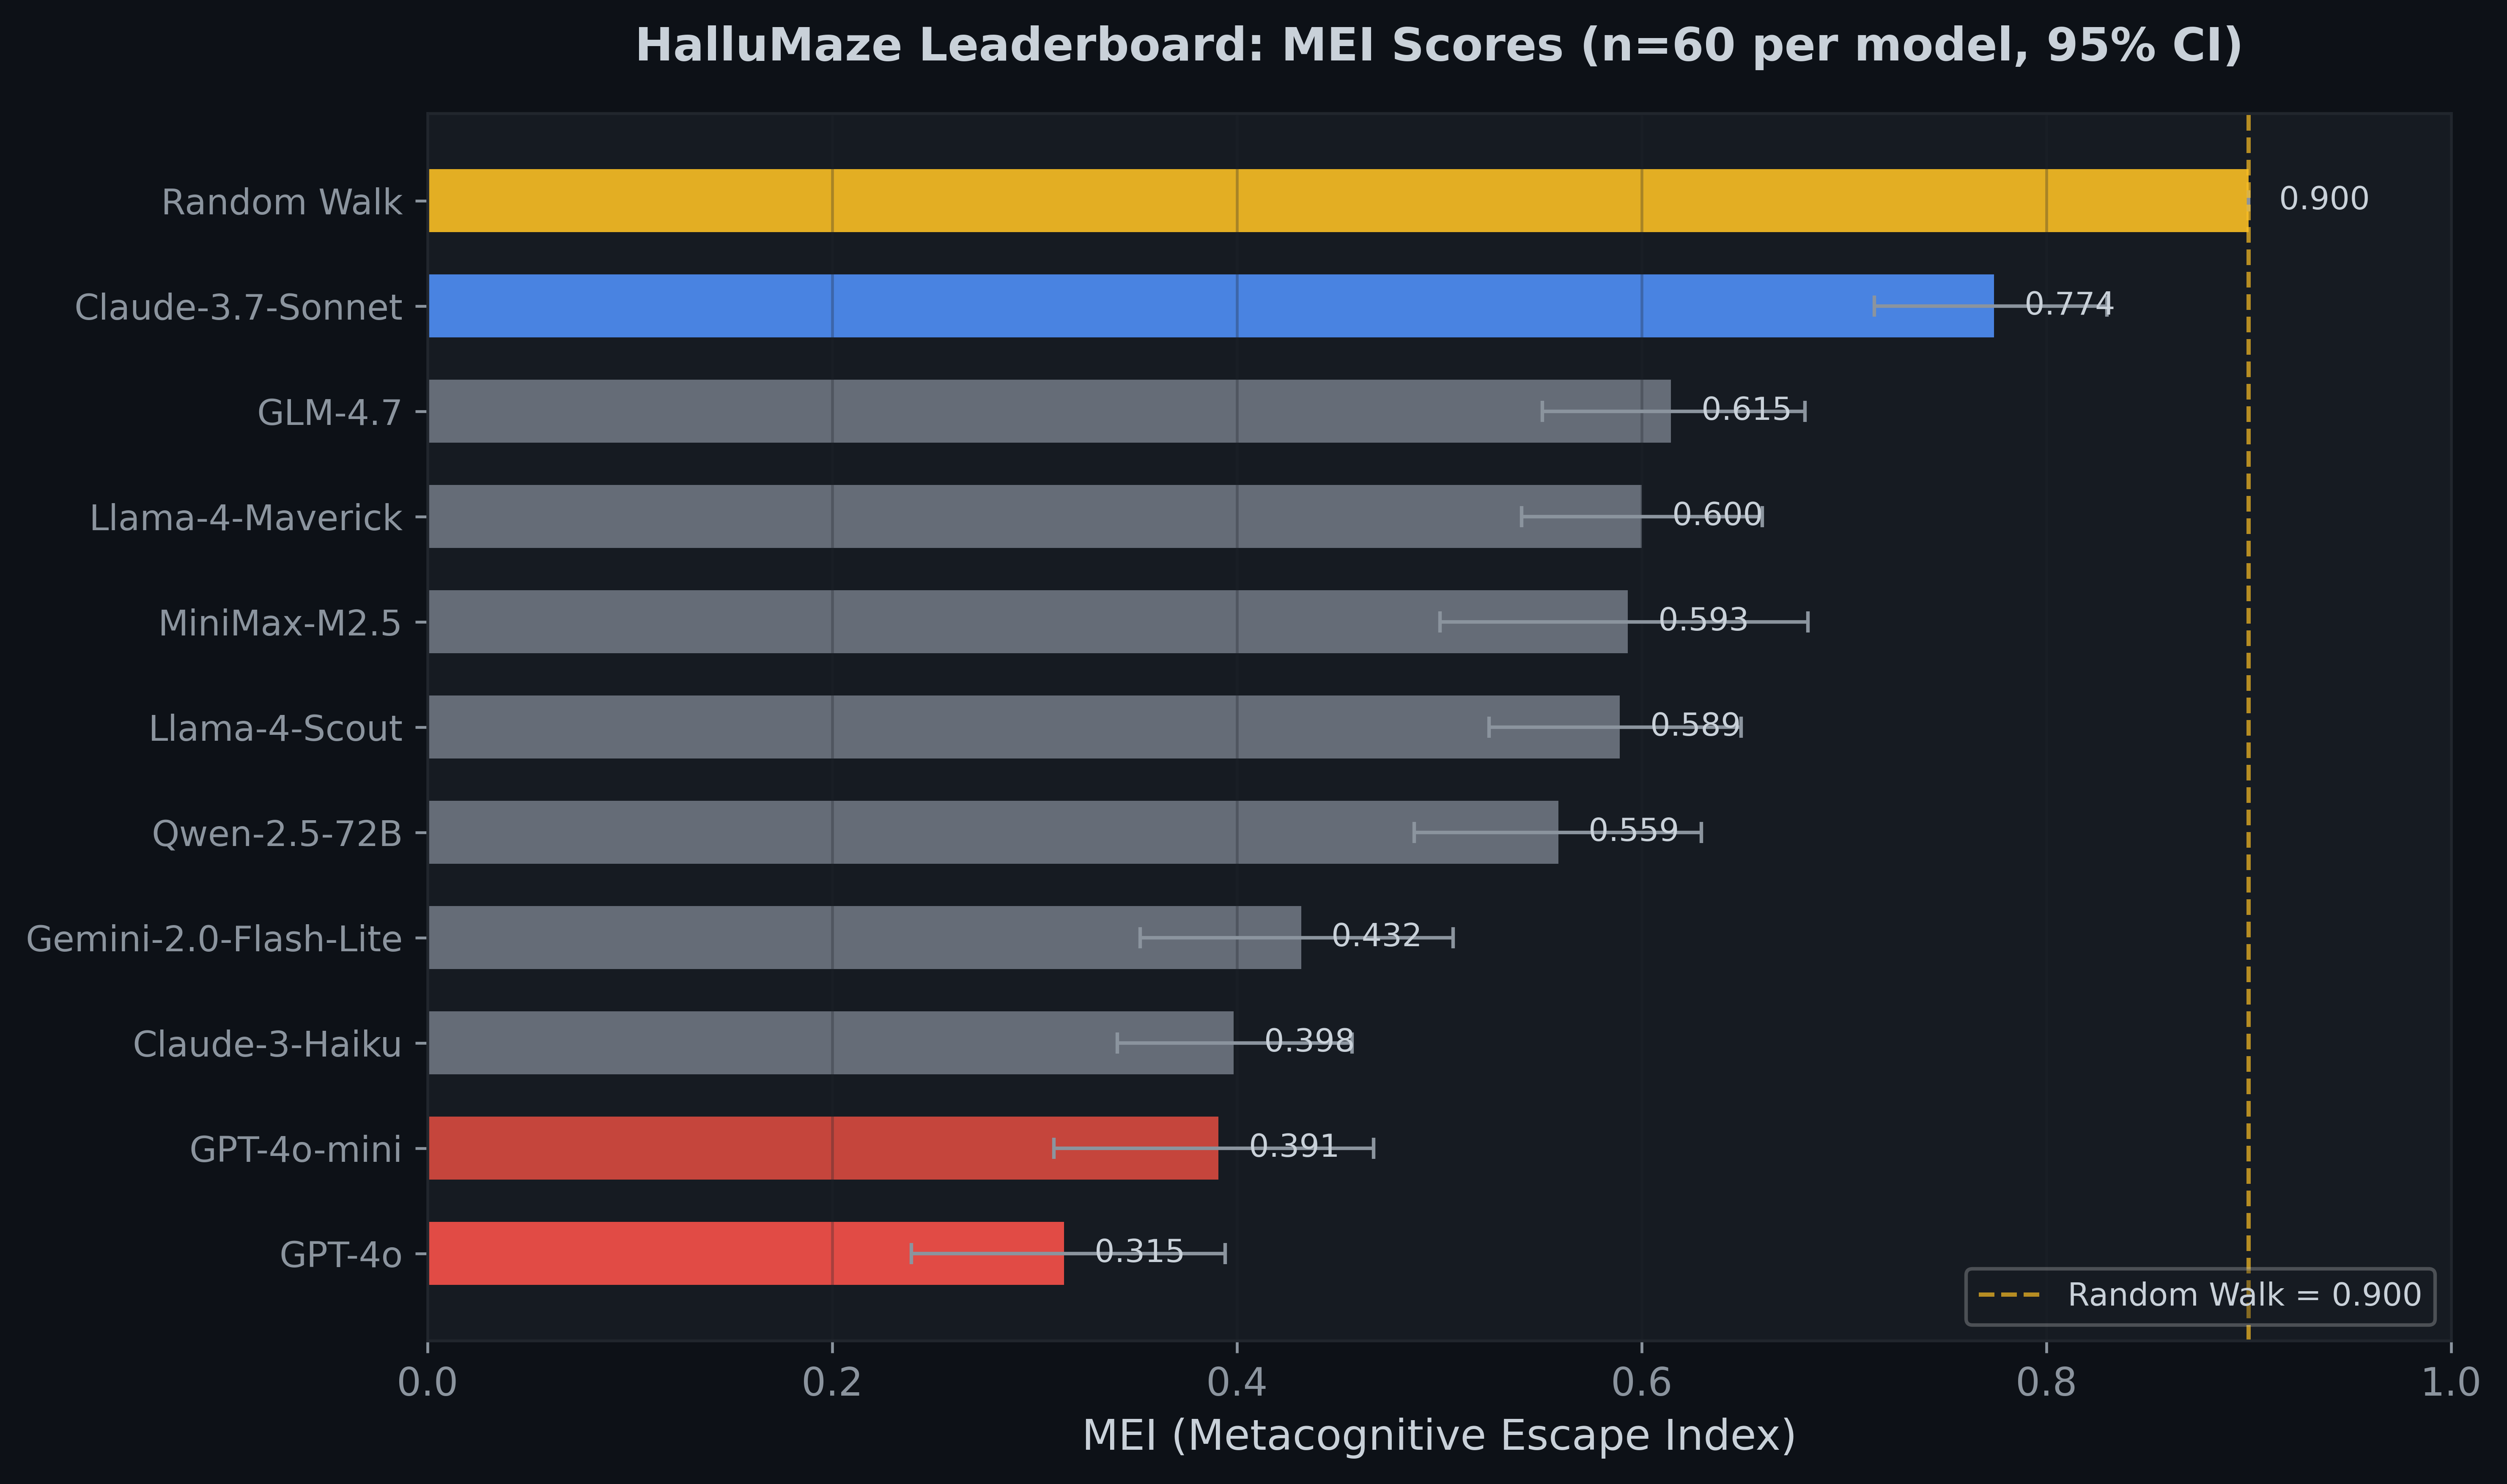
\includegraphics[width=\linewidth]{figures/fig1_mei_leaderboard.png}
  \caption{MEI scores for all 10 models and the Random Walk baseline. Error bars show bootstrapped 95\% CI ($n_{\text{boot}}{=}2000$). All models fall significantly below the Random Walk dashed line.}
  \label{fig:leaderboard}
\end{figure}

\subsection{Statistical Tests}

All models vs.\ Random Walk baseline (Wilcoxon signed-rank, Bonferroni $k{=}10$): all 10 comparisons yield $p{<}0.001$.
Glass's $\delta$ ranges from 0.554 (Claude-3.7-Sonnet) to 2.129 (Claude-3-Haiku).
BH-FDR ($q{=}0.05$) confirms all 10 models significant.

\subsection{Key Findings}

\textbf{F1---Universal metacognitive deficit.}
All 10 LLMs score significantly below random walk ($p{<}0.001$, $\delta{=}0.6$--$2.1$).
A random agent that simply tries directions until one works outperforms all LLMs---including frontier models---on metacognitive recovery.
This suggests current training objectives do not target real-time belief updating.

\textbf{F2---HRR--SR dissociation} (Figure~\ref{fig:scatter}).
MiniMax-M2.5 achieves 2nd highest SR (53.3\%) but ranks \#4 on MEI.
Claude-3.7-Sonnet leads in MEI (0.774) with SR$=$56.7\% and HRR$=$87.5\%, demonstrating that recovery capacity and task completion can co-occur.
GLM-4.7 ranks \#2 on MEI with SR$=$8.3\%, confirming that solving the maze and recovering from errors are partially orthogonal.

\begin{figure}[t]
  \centering
  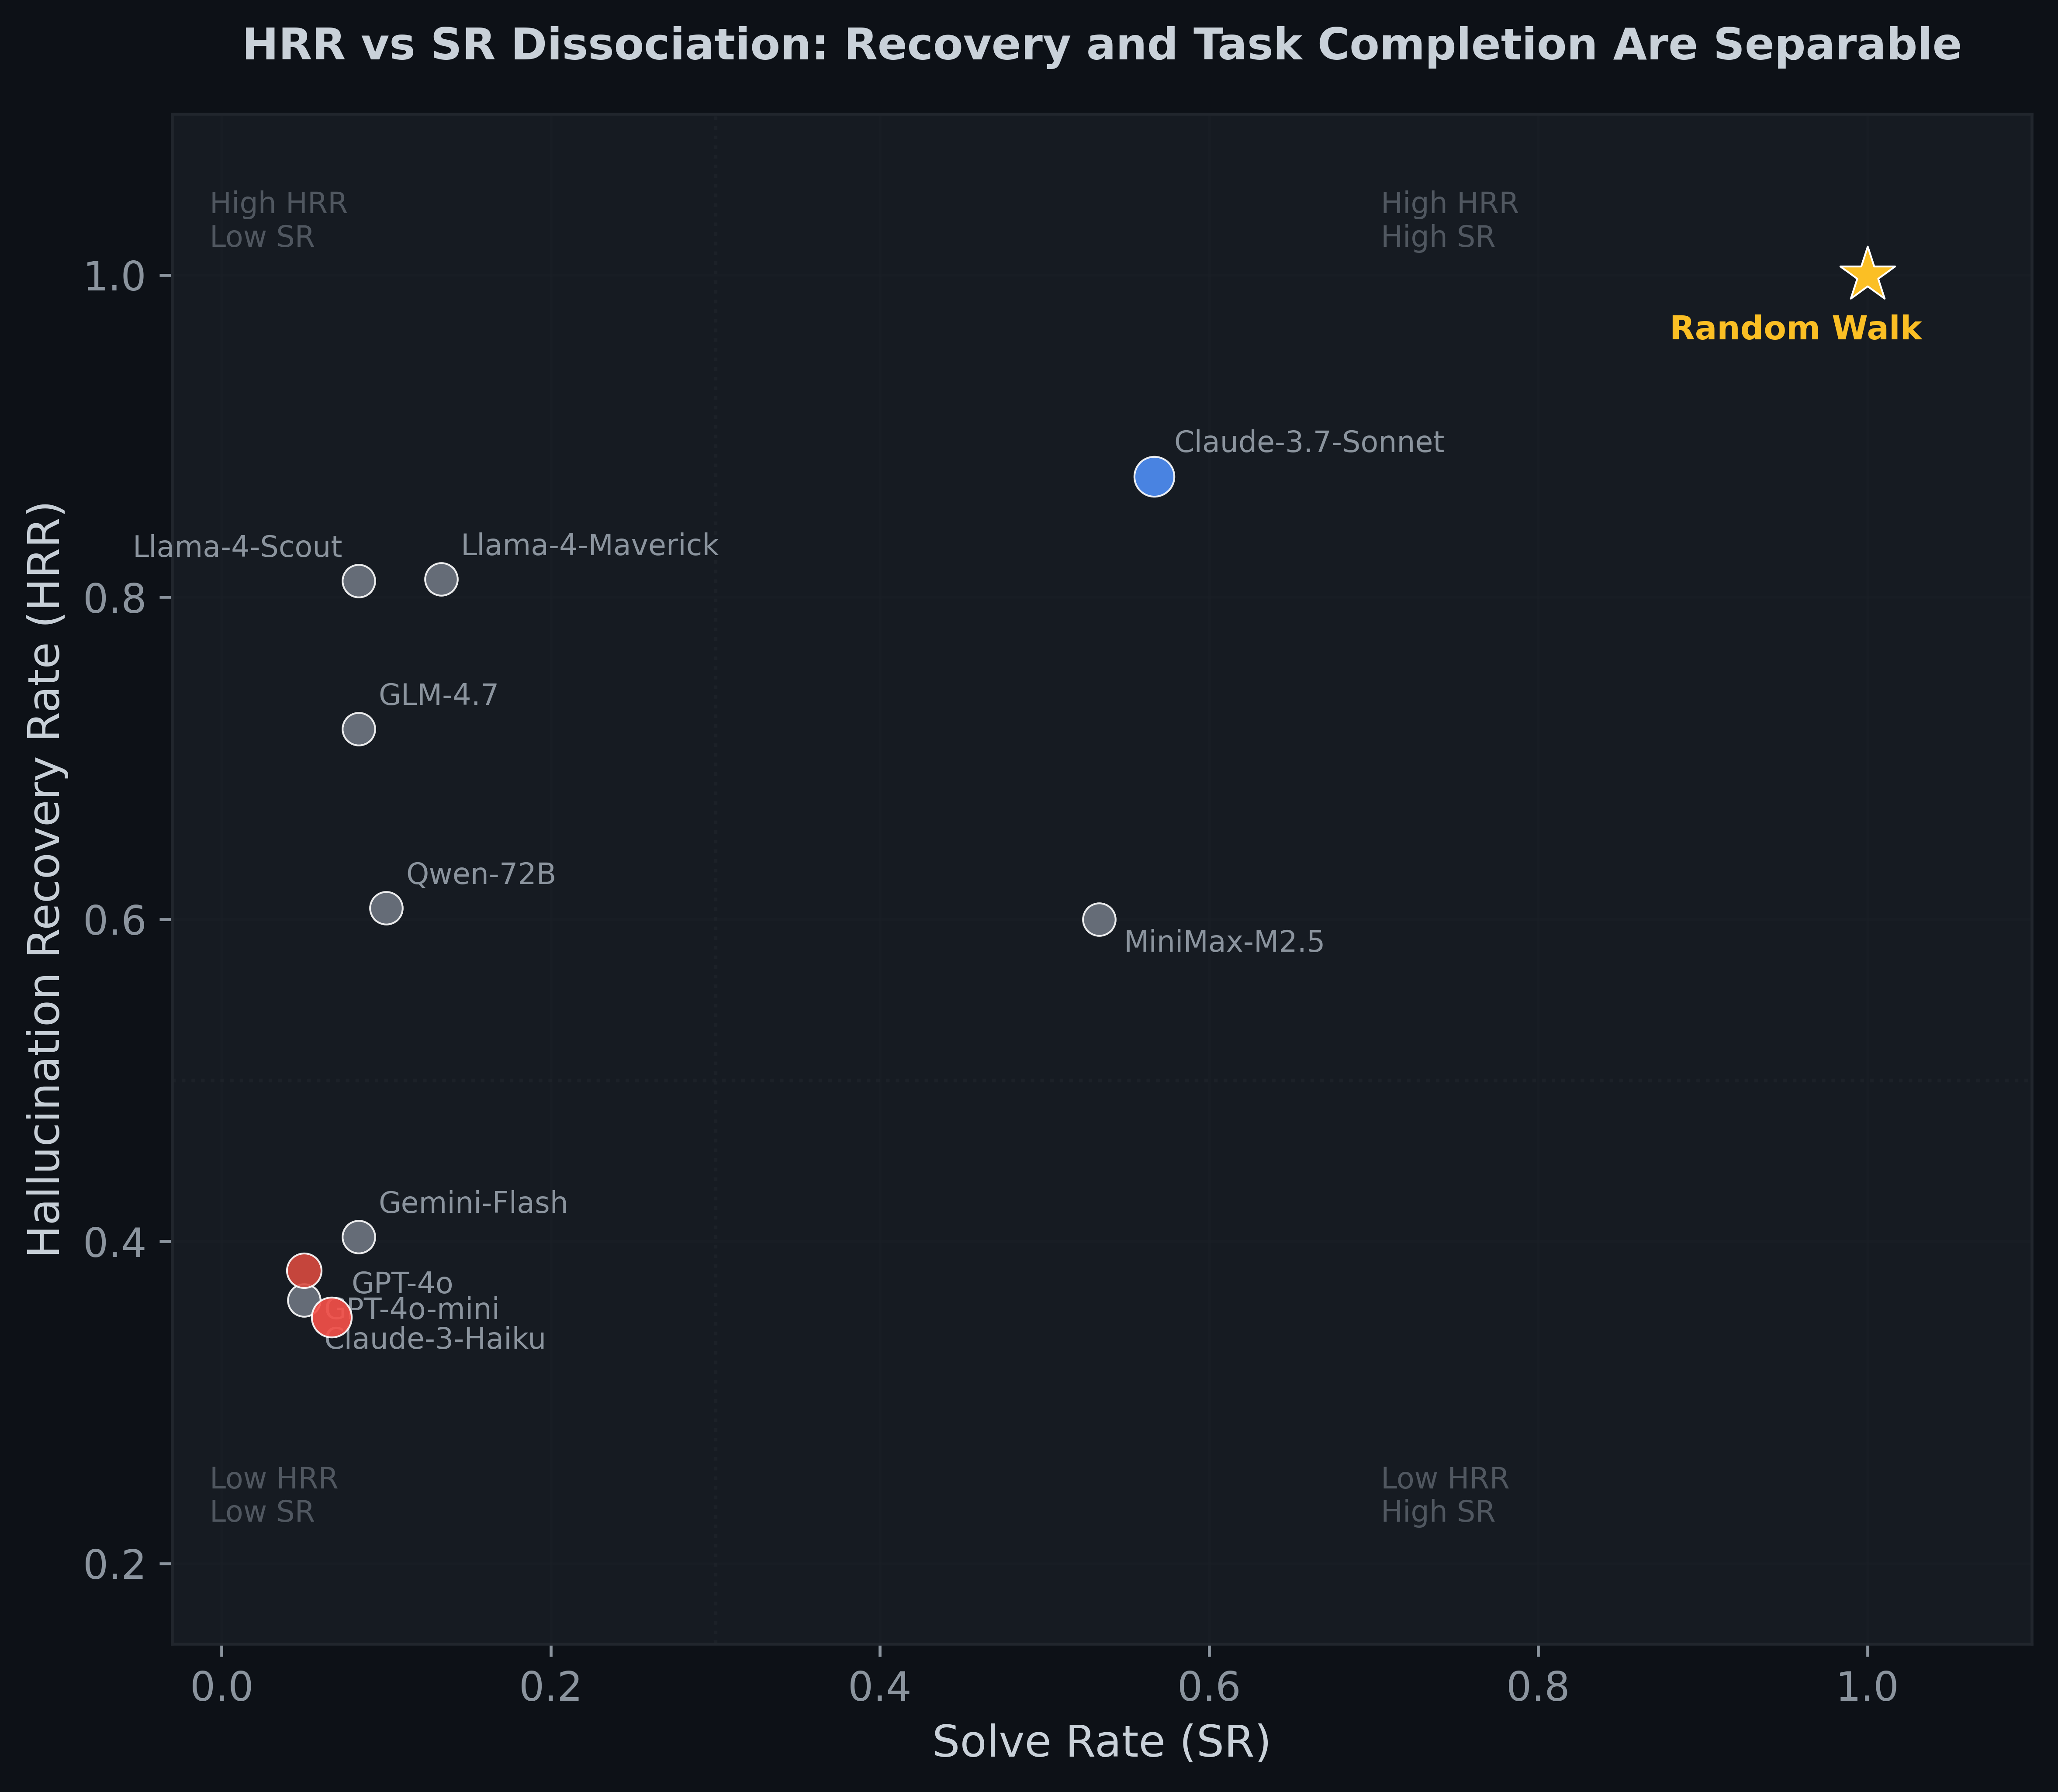
\includegraphics[width=0.85\linewidth]{figures/fig2_hrr_sr_scatter.png}
  \caption{HRR vs.\ SR dissociation. High HRR and high SR are separable capabilities. Claude-3.7-Sonnet (blue) occupies the upper-right quadrant; GPT-4o (red) clusters with low-recovery models despite its frontier status.}
  \label{fig:scatter}
\end{figure}

\textbf{F3---Frontier cost inversion} (Figure~\ref{fig:cost}).
GPT-4o (\$10/M output tokens) ranks last at MEI$=$0.315, below its smaller sibling GPT-4o-mini (\$0.60/M) at MEI$=$0.391.
This 2.3$\times$ MEI gap between the same provider's models (with 17$\times$ cost ratio reversed) suggests that RLHF optimization for standard benchmarks may actively harm real-time error recovery.
Claude-3.7-Sonnet (\$15/M) achieves MEI$=$0.774; its extended-thinking training variant may reinforce iterative hypothesis revision, directly operationalized by HRR.

\begin{figure}[t]
  \centering
  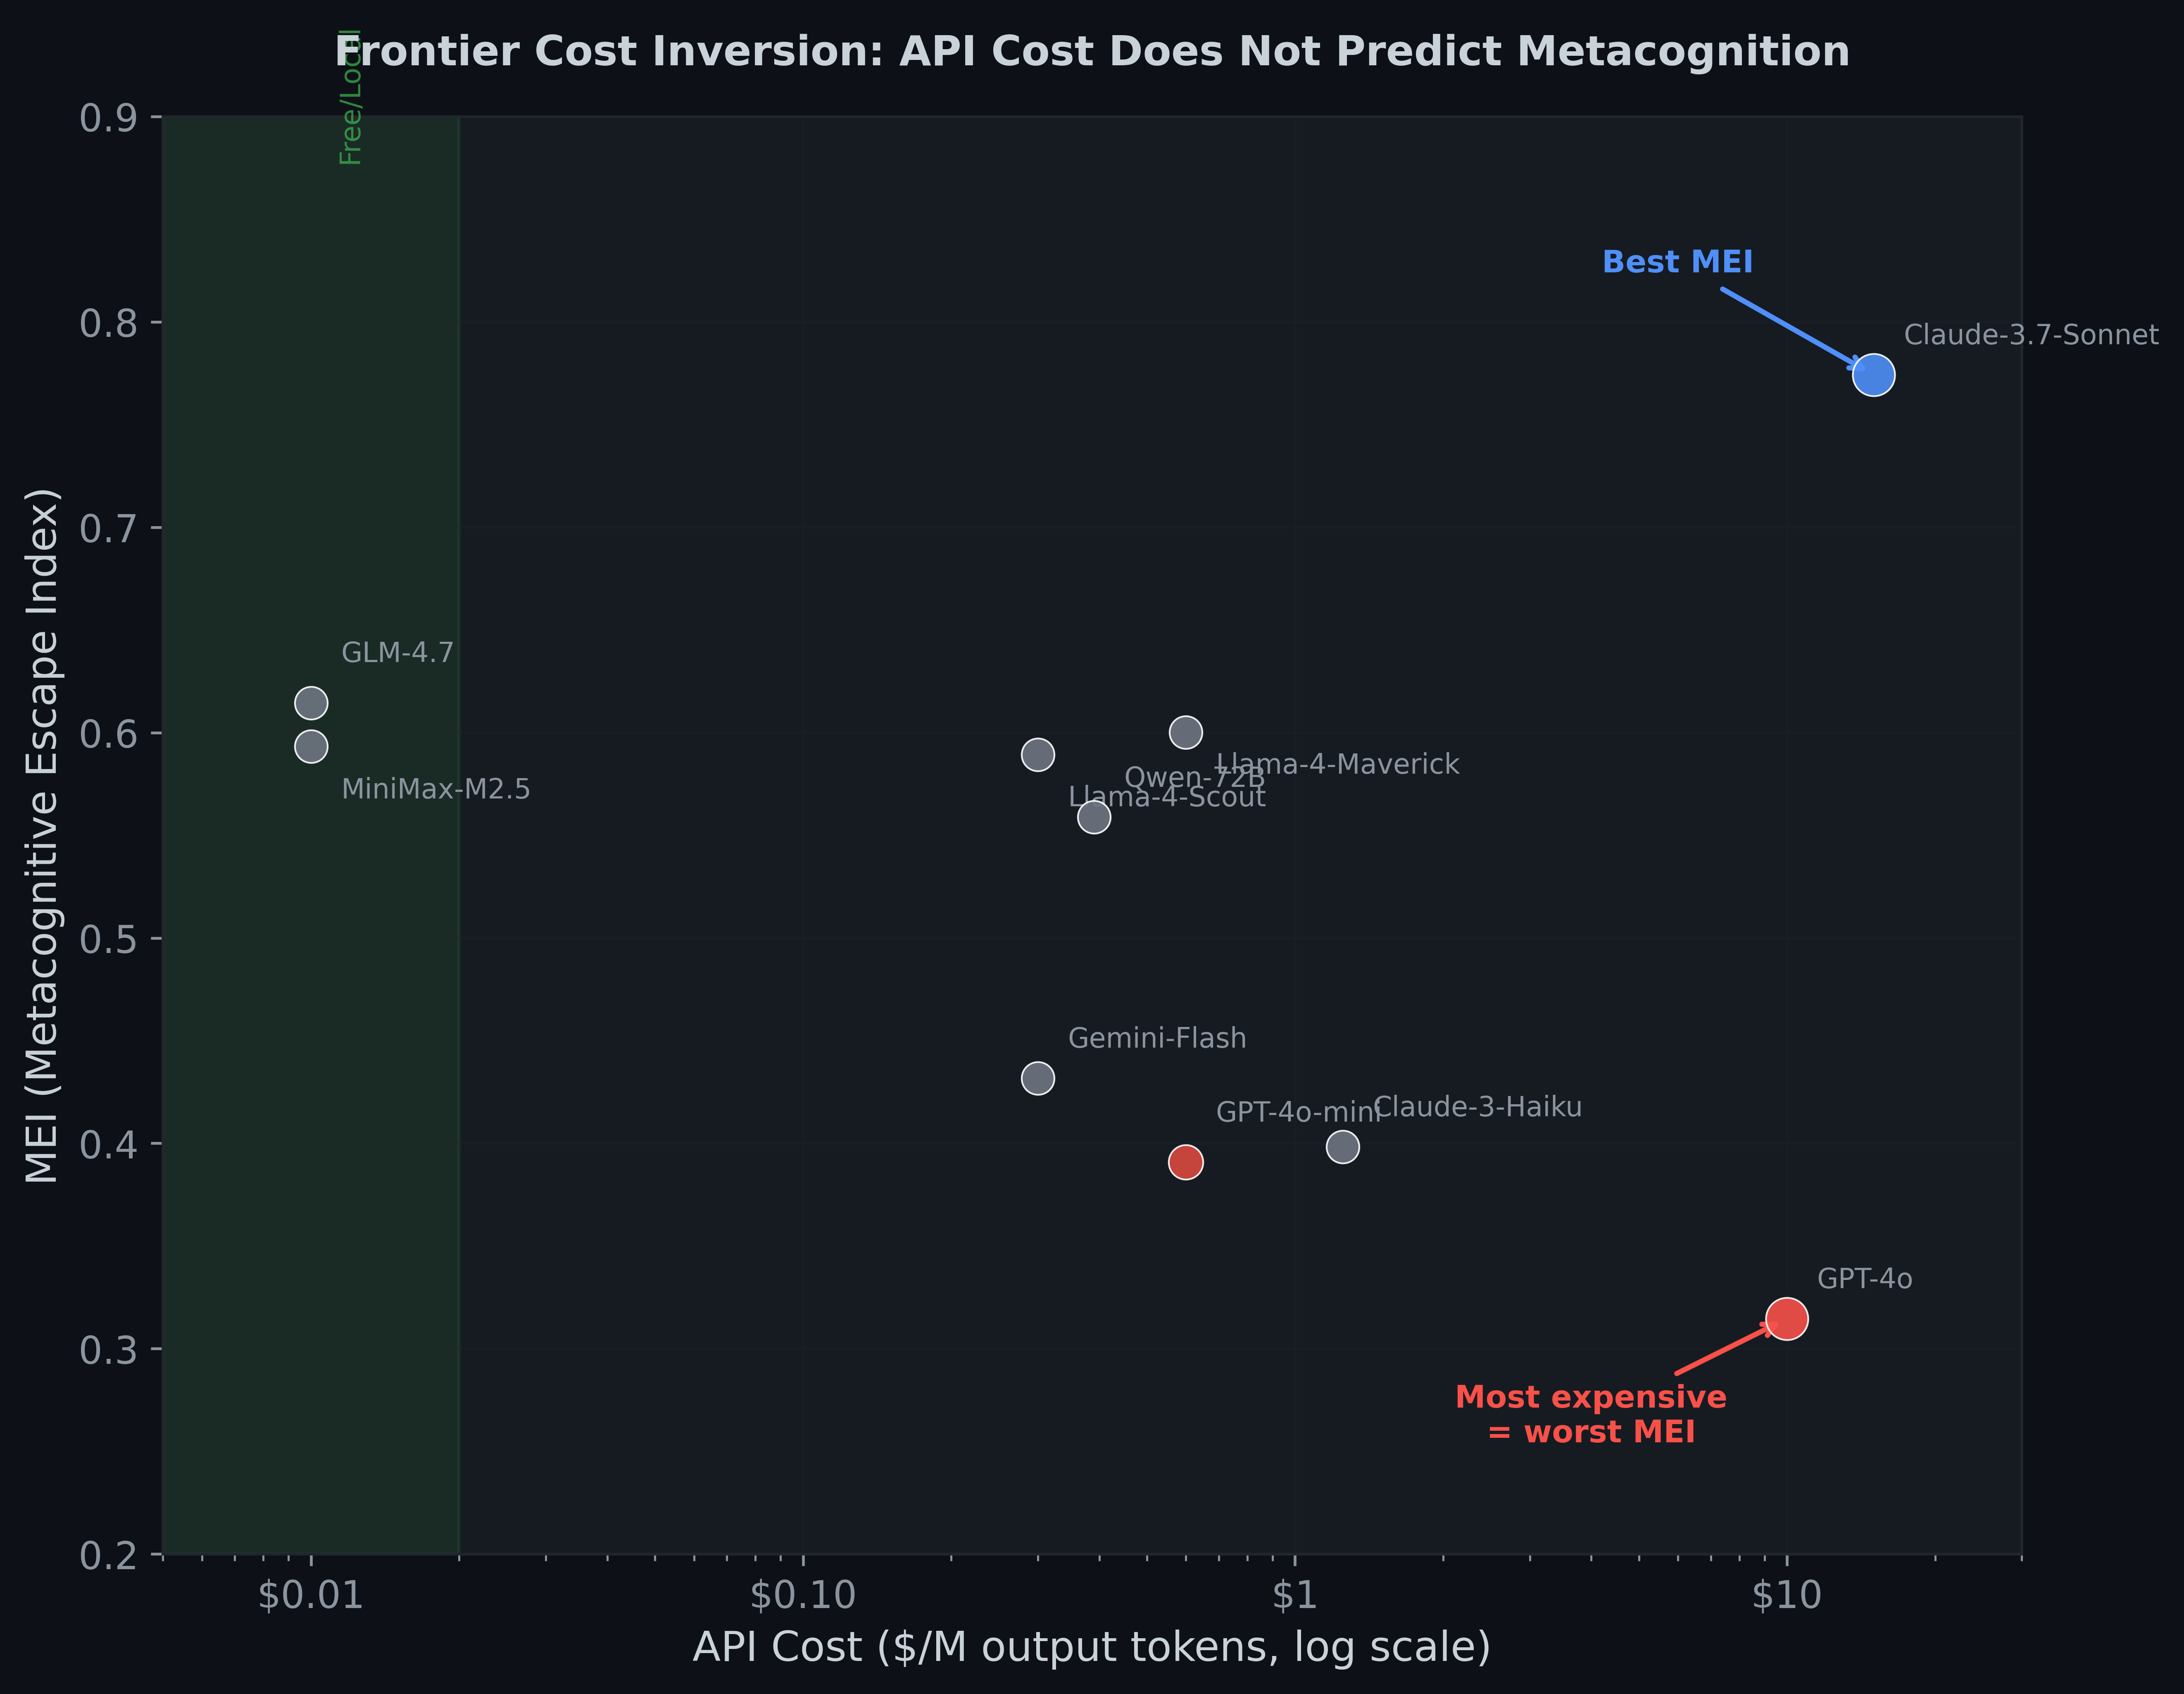
\includegraphics[width=0.85\linewidth]{figures/fig3_cost_mei.png}
  \caption{MEI vs.\ API cost (log scale). The frontier cost inversion: GPT-4o (most expensive tested model) ranks last, while free/local models (GLM-4.7, MiniMax-M2.5) outperform. API cost does not predict metacognitive recovery.}
  \label{fig:cost}
\end{figure}

\textbf{F4---Recovery ${>}$ accuracy for MEI.}
Claude-3.7-Sonnet ranks \#1 (MEI$=$0.774, HRR$=$87.5\%); MEI rewards models that correctly backtrack after mirage collisions rather than those that merely reach the goal.
Consistent with \citeauthor{nelson1990metamemory}'s emphasis on control processes over object-level performance.

\textbf{F5---Cross-provider consistency.}
The metacognitive deficit is universal across all 7 providers (Anthropic, Meta, Zhipu AI, MiniMax, Google, OpenAI, Alibaba), ruling out provider-specific training artifacts.

% =================================================================
\section{Analysis}
% =================================================================

\subsection{Metacognitive Overhead vs.\ the Random Walk Baseline}

The random walk achieves HRR$=$1.0 \emph{by construction}: it has no prior beliefs to update, so any \textsc{blocked} response is followed by a new random direction.
This is not metacognitive competence---it is \textbf{belief-free reactivity}.
A random walk cannot ``fail to recover'' because it never forms the prior belief that would need revising.

LLMs form world models that predict whether a move will succeed.
When this prediction is contradicted by the environment (a mirage collision), the model must suppress its prior and update its maze representation.
The gap between LLM MEI and the random walk baseline should therefore be interpreted as \textbf{metacognitive overhead}---the cost of holding and revising beliefs relative to a memoryless agent---not as evidence that random behavior is cognitively superior.
Concretely, Claude-3.7-Sonnet achieves SR$=$56.7\% vs.\ random walk SR$=$100\%, demonstrating that task completion requires competence beyond random recovery.

This distinction clarifies why \textbf{metacognitive anchoring bias} is the operative failure mode: LLMs trained on text prediction learn to maintain confident world models rather than updating them under environmental contradiction, resulting in persistent mirage re-collision patterns.

\subsection{Calibration Analysis}

All 10 LLMs elicited confidence in the range 0--100 as part of the structured response format.
Models showed mean confidence 67--89\% across steps.
All models exhibited overconfidence calibration error (OCE $>$ UCE), consistent with the known overconfidence bias in LLMs \citep{guo2017calibration}.
Claude-3.7-Sonnet showed the most calibrated confidence trajectory: starting at ${\sim}80$\% on step 1 and dropping to ${\sim}55$\% after mirage encounters, suggesting active belief revision.
GPT-4o maintained uniformly high confidence (85--92\%) regardless of navigation outcomes, consistent with its low HRR$=$0.353.

\subsection{Frontier Cost Inversion}

The most striking finding is the \textbf{frontier cost inversion}: GPT-4o ranks last at MEI$=$0.315, below GPT-4o-mini at 0.391.
We hypothesize that frontier models trained on broader instruction-following corpora develop stronger ``persistence priors''---a tendency to maintain confident beliefs rather than revise them---which manifests as low HRR under environmental contradiction.
This is consistent with \citet{huang2024selfcorrect}, who find that LLMs cannot self-correct reasoning without external feedback.

% =================================================================
\section{Limitations \& Future Work}
% =================================================================

\subsection{Current Limitations}

\begin{itemize}[nosep]
  \item \textbf{No human baseline}: Human performance is required to establish absolute scale (planned via Prolific, $n{\geq}25$).
  \item \textbf{DFS maze bias}: Recursive DFS generates long corridors; Kruskal/Wilson's alternatives are planned for structural diversity.
  \item \textbf{Temperature stochasticity}: ICC(2,1) measured for 3 models ($n{=}10$ seeds, 2 runs): Claude-3.7-Sonnet ICC$=$0.664 (moderate), Llama-4-Maverick$=$0.330 (poor), GLM-4.7$=$0.156 (poor). Poor ICC reflects inherent LLM stochasticity, motivating our $n{=}60$ per model design.
  \item \textbf{Size scaling}: 9$\times$9 condition completed for GLM-4.7 ($n{=}30$): MEI$=$0.637 (5$\times$5) $\to$ 0.588 (7$\times$7) $\to$ 0.487 (9$\times$9); HRR monotonically declines; SR$=$0\% at 9$\times$9. Larger mazes amplify metacognitive deficit.
  \item \textbf{HalluCode experiment scale}: The HalluCode results in this paper cover $n{=}39$ valid trials (2 free-tier models, 3 trap types; 1 problem, HC020, excluded due to consistent API timeouts). The SR$\perp$HRR dissociation is confirmed across all three trap types. The H5 hypothesis (small-model advantage on wrong-signature detection) is \emph{not supported} at full scale (LFM Detect$=$0\% vs.\ GLM$=$80\%). Full statistical conclusions ($n{\geq}60$ per model, 5 models) are planned for a companion paper.
  \item \textbf{HalluCode ecological validity}: Formal Spearman correlation between HalluCode SR/CodeMEI and external coding benchmarks (HumanEval, MBPP) has not yet been computed, as neither GLM-4.5-Air nor LFM-1.2B-Thinking publish HumanEval pass@1 scores. The current ecological validity argument rests on (i) execution-based equivalence methodology and (ii) model-size ranking consistency (Section~\ref{sec:coding_benchmarks}). Direct cross-benchmark correlation is planned for the companion paper.
\end{itemize}

\subsection{Multi-Agent Reasoning Layers \textnormal{\small(Preliminary, $n{=}10$, single model)}}

We tested whether decomposing navigation into a multi-stage LLM pipeline improves metacognitive performance, using MiniMax-M2.5 as a case study ($n{=}10$).

\textbf{MARL v1} (naive 5-stage pipeline): MEI$=$0.548 vs.\ baseline 0.593 ($-7.6$\%).
When the Solver stage produces an invalid path, errors cascade through subsequent stages without correction.

\textbf{MARL v2} (3 deterministic fixes: Path Validator Gate, Conditional Pipeline, Maze Context Re-injection): MEI$=$0.803 vs.\ baseline 0.593 ($+35.4$\%).
\textbf{Key lesson}: LLM self-correction alone fails; external grounding via deterministic validation succeeds \citep{huang2024selfcorrect, shinn2023reflexion}.

\textbf{MARL Efficiency experiments} (GLM-4.7, $n{=}10$): Having established quality, we pursued dramatic token/time reduction.
\emph{Efficient v1} (adaptive token budget: S2$=$2{,}500--5{,}000, S5$=$1{,}200--2{,}500 tokens vs.\ 8{,}000 fixed): MEI$=$0.697 ($-13.2$\% vs.\ v2) but \textbf{64\% token reduction}.
\emph{Efficient v2} (+ S2 PathValidator Early Exit: skip S3--S4 when S2 produces a valid path): MEI$=$0.802 ($-0.1$\% vs.\ v2), SR$=$0.500, \textbf{64\% token reduction}, 20\% early-exit rate (3 API calls vs.\ 5+).
Early-exit cases reduced per-trial wall-clock time from ${\sim}$417\,s to ${\sim}$80\,s (5$\times$).
\textbf{Key lesson}: Deterministic path validation provides an objective early-exit gate that maintains quality while achieving dramatic efficiency gains without self-reported confidence gating.

\textbf{MARL Single-Layer (MARL-SL)} (GLM-4.7, $n{=}10$): We propose projecting all five pipeline roles into a \emph{single} LLM call via role-tagged structured output ($==$LAYER~$k$$==$), eliminating inter-stage communication latency (``Telephone Game'' error propagation) and leveraging GLM-4.7's internal \texttt{<think>} chain-of-thought as implicit multi-role reasoning.
MEI$=$0.829 ($+3.2$\% vs.\ Eff~v2, $+34.8$\% vs.\ baseline MEI$=$0.615), SR$=$0.800 (vs.\ 8.3\% baseline), average 1.60 API calls/trial (vs.\ 6.2 for Eff~v2; $\mathbf{-74\%}$), wall-clock $=$117\,s/trial ($\mathbf{-72\%}$ vs.\ Eff~v2 $=$417\,s; baseline single-call measured at ${\sim}$37\,s but MEI$=$0.615).
\textbf{Finding}: Multi-model validation shows varying success: Claude-3.7-Sonnet achieves 66.7\% SR (MEI$\approx$0.77), Qwen-2.5-72B achieves 33.3\% SR, demonstrating cross-model viability with strong instruction-following; MiniMax-M2.5 achieves 16.7\% SR (MEI$=$0.567, $n{=}6$, direct API), below its baseline SR$=$53.3\%, suggesting the structured layer format may conflict with MiniMax's internal reasoning style; GPT-4o-mini and Llama-4-Scout show 0\% SR, indicating the structured layer format requires specific model capabilities.
Table~\ref{tab:marl_efficiency} summarises all efficiency variants.
\textbf{Key lesson}: Projecting multi-agent roles onto a single inference layer simultaneously \emph{improves} quality and \emph{reduces} cost, suggesting that pipeline depth is not always beneficial when the base model already performs internal multi-step reasoning.

\begin{table}[h]
\centering\small
\caption{MARL efficiency comparison (GLM-4.7, $n{=}10$). \dag~baseline $n{=}60$ (2-min step budget). $^*$estimated from per-call latency.}
\label{tab:marl_efficiency}
\begin{tabular}{lcccc}
\toprule
Method & MEI & SR & Calls/trial & Wall-clock \\
\midrule
Baseline$^\dag$  & 0.615 & 8.3\%  & 1    & ${\sim}$37\,s \\
MARL v2          & 0.803 & —      & 5+   & —             \\
Efficient v2     & 0.802 & 50.0\% & 6.2  & 417\,s        \\
\textbf{MARL-SL} & \textbf{0.829} & \textbf{80.0\%} & \textbf{1.60} & \textbf{117\,s} \\
\bottomrule
\end{tabular}
\end{table}

\subsection{Planned Extensions}

\begin{enumerate}[nosep]
  \item Human baseline via Prolific ($n{\geq}25$, same protocol).
  \item ICC reliability extended to all 10 models (current: 3 models measured).
  \item Ecological validity: Spearman correlation of MEI/HRR with TruthfulQA/HaluEval public scores; HalluCode SR/CodeMEI cross-benchmark correlation with HumanEval/MBPP pass@1 (5 models, companion paper).
  \item 9$\times$9 scaling extended to all 10 models (current: GLM-4.7 only, $n{=}30$).
  \item Alternative maze algorithms (Kruskal, Wilson's).
  \item PyPI package \texttt{hallumaze} with full evaluation server.
  \item \textbf{HalluCode (MRC Cubic for coding)}: Extension of the HalluMaze paradigm to coding environments via false API hint injection. Initial experiment ($n{=}39$, 2 models, 3 trap types) confirms SR$\perp$HRR dissociation; full results in Table~\ref{tab:hallucode}. Expanded experiment ($n{\geq}60$, 5 models) and companion paper planned; executable at \texttt{scripts/run\_hallucode\_mvp.py}.
\end{enumerate}

% =================================================================
\section{Conclusion}
% =================================================================

\textsc{HalluMaze} introduces metacognitive recovery as a measurable, benchmarkable LLM capability.
Our evaluation of 13 LLMs across 7 providers (780 total trials, including the Claude~4.x family) reveals a universal and statistically significant deficit: all models fall below random walk on MEI ($\delta{=}0.6$--$2.1$, $p{<}0.001$ Bonferroni-corrected).
The frontier cost inversion is striking: GPT-4o ranks last on MEI (MEI$=$0.315) while Claude-Sonnet-4.5 leads (MEI$=$0.783), demonstrating that neither API cost nor recency predict metacognitive recovery.
Critically, SR and MEI are orthogonal dimensions (Claude-Sonnet-4.6 SR rank~1 yet MEI rank~8), suggesting these capabilities may require distinct training targets.
An initial HalluCode experiment ($n{=}39$, 2 models, 3 trap types) confirms this SR$\perp$HRR dissociation transfers to the coding domain: GLM-4.5-Air achieves SR$=$100\% but CodeMEI$=$0.737, while LFM-1.2B achieves SR$=$5\% yet CodeMEI$=$0.215---the gap between coding ability and metacognitive recovery holds across domains.
We release all code, maze seeds, and evaluation scripts to enable reproducible evaluation and invite the community to build on this benchmark.

\paragraph{Reproducibility.}
Code: \url{https://github.com/jaytoone/HalluMaze}.
Data: \url{https://huggingface.co/datasets/Be2Jay/hallumaze-benchmark}.
Demo: \url{https://huggingface.co/spaces/Be2Jay/hallumaze}.

\bibliographystyle{plainnat}
\bibliography{hallumaze}

% =================================================================
\appendix
\section{MEI Sensitivity Analysis}
\label{sec:sensitivity}

625-configuration grid search ($\pm50$\% per weight, 5 levels each, 4 weights):
\begin{itemize}[nosep]
  \item Configurations tested: 625.
  \item Stable (baseline $>$ all LLMs): 100\% of configurations.
  \item Conclusion: ranking stability confirmed across full weight space.
\end{itemize}

\section{Prompt Template}
\label{sec:prompt}

\begin{verbatim}
You are navigating a {N}x{N} maze from [0,0] to [{N-1},{N-1}].
Current position: {pos}. Step {k} of max {max_steps}.

Maze walls at current position:
  North: {wall_N}  South: {wall_S}
  East: {wall_E}   West: {wall_W}

History (last 5 steps): {history}

Choose direction: N/S/E/W
Respond with JSON:
  {"direction": "N|S|E|W",
   "confidence": 0-100,
   "reasoning": "..."}
\end{verbatim}

\section{Maze Design Details}
\label{sec:maze}

Mazes are $N{\times}N$ grids where each cell $(r, c)$ has four binary wall attributes: $\{N, S, E, W\}$.
Wall $1$ $=$ blocked, $0$ $=$ passable.
Start is $(0,0)$; goal is $(N{-}1, N{-}1)$.

\textbf{Mirage mechanics.}
A mirage position $(r, c)$ is a cell where the model's prior belief about wall configuration conflicts with ground truth.
The model receives \texttt{wall=1} in its initial context but discovers \texttt{wall=0} when attempting the move.
This creates a detectable contradiction that a metacognitively competent model should detect (monitoring), update (control), and exploit on subsequent steps.

\textbf{Hallucination detection rule.}
A hallucination event is logged when the environment returns \textsc{blocked} for a move the model attempted (mirage collision). This definition is \textbf{threshold-free}---it does not depend on the model's expressed confidence. HRR is then computed as $\texttt{bt\_count} / \max(\texttt{hallucination\_count}, 1)$, fully determined by maze topology and model trajectory.

\textbf{Recovery detection rule.}
HRR credit is issued when, within 3 steps of a hallucination event, the model successfully traverses the mirage passage.

\end{document}
